%! Author = joels
%! Date = 24/12/2020

\section{Functions and Exceptions}
% You can choose the most suitable way to take parameters in functions
% You know how to write a lambda with a capture
% You know 5 different ways to react to errors in functions
% You know how to throw , catch and test exceptions

\subsection{Functions}
\begin{center}
    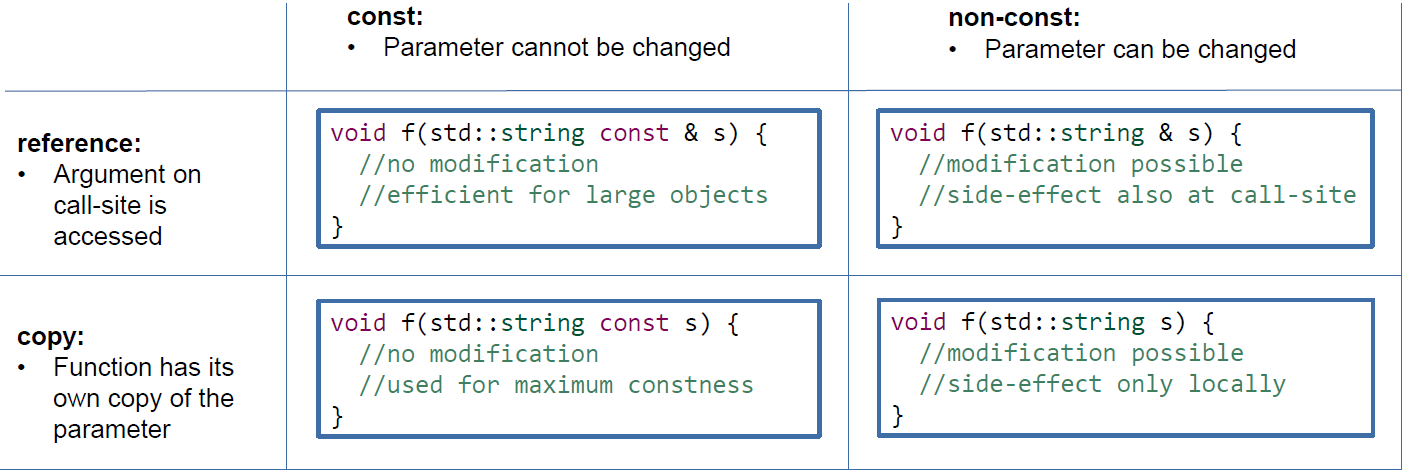
\includegraphics[scale=0.42]{function_parameter_declarations.png}
\end{center}

\subsubsection{When to use \& and const Parameters:}
\begin{itemize}
    \item Value Parameter:
    \SubItem{Default case}
    \item Reference Parameter
    \SubItem{When side-effect is required at call-site}
    \item Const-Reference Parameter
    \SubItem{Possible optimization, when type is large (costly to copy) and no side effects desired at call site}
    \SubItem{For non-copyable objects}
    \item Const Value Parameter
    \SubItem{The coding style guide of your project this might prefer this over non const value parameters}
    \SubItem{Could prevent changing the parameter in the function inadvertently}
\end{itemize}

\subsubsection{Function Overloading}
The same function name can be used for different functions if parameter number or types differ\\
$\rightarrow$ Functions cannot be overloaded just by their return type\\
$\rightarrow$ If only the parameter type is different there might be ambiguities
\subsubsection{Default Arguments}
\begin{itemize}
    \item A function declaration can provide default arguments for its parameters from the right.
    \SubItem{E.g: \textcolor{blue}{void incr(int \& var, unsigned delta = 1);}}
    \item Implicit overload of the function with fewer parameters
        \SubItem{If n default arguments are provided, n+1 versions of the function are declared}
    \item Default arguments can be omitted when calling the function
\end{itemize}

\subsubsection{Functions as Parameters}
Functions are \dq first class\dq objects in C++\\
$\rightarrow$ You can pass them as argument, or keep them in reference variables.

\begin{lstlisting}[style=frame, style= linenumbers, language=C]
// As Argument (No Lambads/Captures before function allowed)
void applyAndPrint(double x, double f(double)) {
    std::cout << "f(" << x << ") = " << f(x) << '\n'; }

// As reference variable
double (&h)(double);

// std::function: template for Lambdas --> #include <functional>
void applyAndPrint(double x, std::function<double(double)> f) {
    std::cout << "f(" << x << ") = " << f(x) << '\n'; }
int main() {
    double factor{3.0};
    auto const multiply = [factor](double value() { // Lambda Function
        return factor * value; };
    applyAndPrint(1.5, multiply);
\end{lstlisting}

\subsection{Failing Functions}
What should you do, if a function cannot fulfill its purpose?
\begin{itemize}
    \item Ignore the error and provide potentially \textcolor{red}{undefined behavior}
    \item Return a standard result to cover the error
    \item Return an error code or error value
    \item Provide an error status as a side-effect
    \item Throw an exception
\end{itemize}

\begin{minipage}{0.5\linewidth}
    \subsubsection{Ignore the error:}
    \begin{itemize}
        \item Relies on the caller to satisfy all preconditions
        \item Most efficient implementation (no unnecessary checks)
        \item Simple for implementer, harder for caller
        \item Should be done consciously and consistently!
    \end{itemize}
    \subsubsection{Error Value}
    \begin{itemize}
        \item Only feasible if result domain is smaller than return type
        \item E.g: Error Value for strings: \textcolor{blue}{std::string::npos}
        \item Optional as return type can contain no value. \\
            $\rightarrow$ \#include$<$optional$>$\\
            E.g: \textcolor{blue}{std::optional$<$std::string$>$}
            \SubItem{caller side: has to check with: \textcolor{blue}{var.has\_value()}}
    \end{itemize}
\end{minipage}
\begin{minipage}{0.5\linewidth}
    \subsubsection{Return standard result:}
    \begin{itemize}
        \item Reliefs the caller from the need to care if it can continue with the default value
        \item Can hide underlying problems
        \item Often better if caller can specify its own default value
    \end{itemize}
    \subsubsection{Error Status}
    \begin{itemize}
        \item Requires reference parameter
        \item Alternative: Global Variable (BAD decision)
        \item E.g: std::istreams's states (good(), fail()) is changed as a side-effect of input
    \end{itemize}
    \subsubsection{Exceptions}
    \begin{itemize}
        \item Prevent execution of invalid logic by throwing an exception
    \end{itemize}
\end{minipage}

\subsection{Exceptions}
Principle: Throw by value, catch by const reference.\\
Functions can be declared to explicitly not throw an exception with the keyword \textcolor{blue}{noexcept}\\
\textcolor{blue}{\textbf{\#include $<$stdexcept$>$}}
\begin{center}
    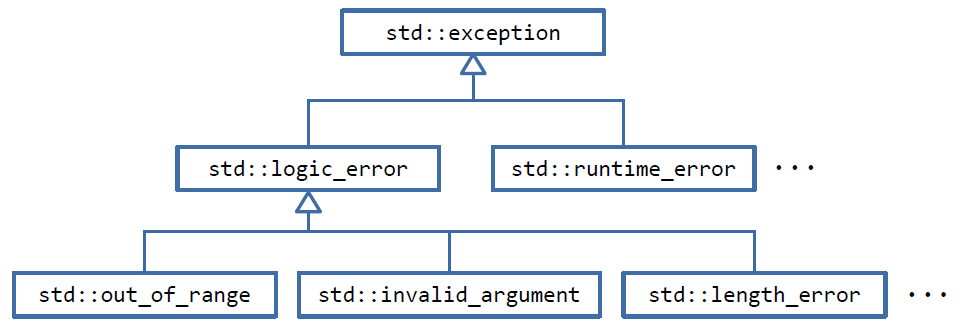
\includegraphics[scale=0.5]{exceptions.png}
\end{center}
\begin{lstlisting}[style=frame, style= linenumbers, language=C]
// Throw an Exception
if (x < 0) {
    throw std::invalid_argument{"square_root imaginary"};
}

// Catch an Exception
try {
    throwingCall();
} catch (type const & e) { /* Handle type exception */
} catch (type2 const & e) { /* Handle type2 exception */
} catch (...) { /* Handle other exception types */
} // Caught exceptions can be rethrown with throw;

//CUTE
void testSquareRootNegativeThrows() {
    ASSERT_THROWS(square_root(-1.0), std::invalid_argument);
}
\end{lstlisting}


